\documentclass[11pt,a4paper]{article}

\usepackage[T1]{fontenc}
\usepackage[utf8]{inputenc}
\usepackage{lmodern}
\usepackage{microtype}
\usepackage[margin=2.6cm]{geometry}
\usepackage{amsmath,amssymb}
\usepackage{booktabs}
\usepackage{graphicx}
\usepackage{caption}
\usepackage{xcolor}
\usepackage[hidelinks]{hyperref}
\usepackage[numbers,sort&compress]{natbib}

\definecolor{fnblue}{HTML}{1F4FE0}
\hypersetup{colorlinks=true,linkcolor=fnblue,citecolor=fnblue,urlcolor=fnblue}
\captionsetup{font=small,labelfont=bf}
\graphicspath{{figures/}}

% generated by make_assets.py, do not edit
\newcommand{\BaseSameWindow}{\ensuremath{-}8.4}
\newcommand{\BnBaseCarry}{10.2}
\newcommand{\BnBaseCost}{4.3}
\newcommand{\BnBaseDD}{\ensuremath{-}32.1}
\newcommand{\BnBaseRet}{42.3}
\newcommand{\BnBaseSharpe}{1.32}
\newcommand{\BnBaseVol}{30.2}
\newcommand{\BnBestXsCarry}{11.1}
\newcommand{\BnBestXsCost}{4.4}
\newcommand{\BnBestXsDD}{\ensuremath{-}26.3}
\newcommand{\BnBestXsRet}{29.4}
\newcommand{\BnBestXsSharpe}{1.35}
\newcommand{\BnBestXsVol}{20.6}
\newcommand{\BnCandCarry}{15.2}
\newcommand{\BnCandCost}{2.2}
\newcommand{\BnCandDD}{\ensuremath{-}2.3}
\newcommand{\BnCandRet}{15.1}
\newcommand{\BnCandSharpe}{5.96}
\newcommand{\BnCandVol}{2.4}
\newcommand{\BnCcCarryTwentyFive}{4.3}
\newcommand{\BnCcCarryTwentyFour}{14.1}
\newcommand{\BnCcCarryTwentyOne}{40.4}
\newcommand{\BnCcCarryTwentyThree}{9.4}
\newcommand{\BnCcCarryTwentyTwo}{3.6}
\newcommand{\BnCcCostEight}{15.1}
\newcommand{\BnCcCostSixteen}{12.6}
\newcommand{\BnCcCostTwentyFour}{10.2}
\newcommand{\BnCcCostZero}{17.6}
\newcommand{\BnCcExcess}{11.9}
\newcommand{\BnCcMonthly}{2.21}
\newcommand{\BnCcNetTwentyFive}{2.4}
\newcommand{\BnCcNetTwentyFour}{12.0}
\newcommand{\BnCcNetTwentyOne}{38.2}
\newcommand{\BnCcNetTwentyThree}{7.4}
\newcommand{\BnCcNetTwentyTwo}{5.9}
\newcommand{\BnCcRet}{15.1}
\newcommand{\BnCcSep}{7.5}
\newcommand{\BnCcTbill}{3.2}
\newcommand{\BnSchedBase}{146}
\newcommand{\BnSchedCc}{1.7}
\newcommand{\BnSchedXsTwentyOne}{46}
\newcommand{\BnWinNeg}{28}
\newcommand{\BnWinWorse}{0.6}
\newcommand{\ByBaseCarry}{7.1}
\newcommand{\ByBaseCost}{4.7}
\newcommand{\ByBaseDD}{\ensuremath{-}22.8}
\newcommand{\ByBaseRet}{32.3}
\newcommand{\ByBaseSharpe}{1.24}
\newcommand{\ByBaseVol}{25.2}
\newcommand{\ByBestXsCarry}{6.6}
\newcommand{\ByBestXsCost}{4.9}
\newcommand{\ByBestXsDD}{\ensuremath{-}22.8}
\newcommand{\ByBestXsRet}{25.9}
\newcommand{\ByBestXsSharpe}{1.40}
\newcommand{\ByBestXsVol}{17.6}
\newcommand{\ByCandCarry}{10.4}
\newcommand{\ByCandCost}{2.7}
\newcommand{\ByCandDD}{\ensuremath{-}0.8}
\newcommand{\ByCandRet}{8.2}
\newcommand{\ByCandSharpe}{6.39}
\newcommand{\ByCandVol}{1.2}
\newcommand{\ByCcCarryTwentyFive}{4.0}
\newcommand{\ByCcCarryTwentyFour}{14.6}
\newcommand{\ByCcCarryTwentyThree}{11.0}
\newcommand{\ByCcCarryTwentyTwo}{5.0}
\newcommand{\ByCcCostEight}{8.2}
\newcommand{\ByCcCostSixteen}{5.3}
\newcommand{\ByCcCostTwentyFour}{2.5}
\newcommand{\ByCcCostZero}{11.1}
\newcommand{\ByCcExcess}{3.7}
\newcommand{\ByCcMonthly}{2.89}
\newcommand{\ByCcNetTwentyFive}{1.1}
\newcommand{\ByCcNetTwentyFour}{11.9}
\newcommand{\ByCcNetTwentyThree}{8.6}
\newcommand{\ByCcNetTwentyTwo}{2.9}
\newcommand{\ByCcRet}{8.2}
\newcommand{\ByCcSep}{4.1}
\newcommand{\ByCcTbill}{4.5}
\newcommand{\BySchedBase}{69}
\newcommand{\BySchedCc}{0.4}
\newcommand{\BySchedXsTwentyOne}{29}
\newcommand{\ByWinNeg}{24}
\newcommand{\ByWinWorse}{0.0}
\newcommand{\CBaseVol}{0.65}
\newcommand{\CCorr}{0.96}
\newcommand{\CDays}{11}
\newcommand{\CTotal}{\ensuremath{-}7.8}
\newcommand{\CVol}{0.67}
\newcommand{\CcDays}{10}
\newcommand{\CcLiveCarry}{\ensuremath{+}0.016}
\newcommand{\CcLiveCarryAnn}{0.6}
\newcommand{\CcLiveCost}{0.115}
\newcommand{\CcLiveTotal}{\ensuremath{-}0.12}
\newcommand{\Dsr}{0.994}
\newcommand{\DsrNull}{4.5}
\newcommand{\HoCcCarryTwentySix}{2.0}
\newcommand{\HoCcCostEight}{\ensuremath{-}1.8}
\newcommand{\HoCcCostSixteen}{\ensuremath{-}5.1}
\newcommand{\HoCcCostTwentyFour}{\ensuremath{-}8.4}
\newcommand{\HoCcCostZero}{1.7}
\newcommand{\HoCcMonthly}{\ensuremath{-}1.59}
\newcommand{\HoCcNetTwentySix}{\ensuremath{-}1.8}
\newcommand{\HoCcRet}{\ensuremath{-}1.8}
\newcommand{\HoCcSep}{\ensuremath{-}0.9}
\newcommand{\HoTauFifteenCost}{0.0}
\newcommand{\HoTauFifteenExcess}{0.0}
\newcommand{\HoTauFifteenGross}{0}
\newcommand{\HoTauFifteenNet}{0.0}
\newcommand{\HoTauFiveCost}{2.2}
\newcommand{\HoTauFiveExcess}{\ensuremath{-}3.6}
\newcommand{\HoTauFiveGross}{45}
\newcommand{\HoTauFiveNet}{\ensuremath{-}1.9}
\newcommand{\HoTauTenCost}{0.2}
\newcommand{\HoTauTenExcess}{\ensuremath{-}0.1}
\newcommand{\HoTauTenGross}{6}
\newcommand{\HoTauTenNet}{\ensuremath{+}0.2}
\newcommand{\HoTauZeroCost}{3.5}
\newcommand{\HoTauZeroExcess}{\ensuremath{-}5.3}
\newcommand{\HoTauZeroGross}{96}
\newcommand{\HoTauZeroNet}{\ensuremath{-}1.8}
\newcommand{\HoldBaseCarry}{3.1}
\newcommand{\HoldBaseCost}{5.5}
\newcommand{\HoldBaseSharpe}{0.16}
\newcommand{\HoldBaseTotal}{\ensuremath{+}0.4}
\newcommand{\HoldBestPairCarry}{0.0}
\newcommand{\HoldBestPairCost}{4.0}
\newcommand{\HoldBestPairSharpe}{\ensuremath{-}1.50}
\newcommand{\HoldBestPairTotal}{\ensuremath{-}11.9}
\newcommand{\HoldBestXsZeroCarry}{3.6}
\newcommand{\HoldBestXsZeroCost}{4.3}
\newcommand{\HoldBestXsZeroSharpe}{\ensuremath{-}1.68}
\newcommand{\HoldBestXsZeroTotal}{\ensuremath{-}11.0}
\newcommand{\HoldBestXscCarry}{4.2}
\newcommand{\HoldBestXscCost}{5.1}
\newcommand{\HoldBestXscSharpe}{\ensuremath{-}1.82}
\newcommand{\HoldBestXscTotal}{\ensuremath{-}11.9}
\newcommand{\HoldCandCarry}{2.0}
\newcommand{\HoldCandCost}{3.5}
\newcommand{\HoldCandSharpe}{\ensuremath{-}1.50}
\newcommand{\HoldCandTotal}{\ensuremath{-}0.7}
\newcommand{\HoldSchedHi}{\ensuremath{+}31.0}
\newcommand{\HoldSchedLo}{\ensuremath{-}32.2}
\newcommand{\HoldSchedMed}{\ensuremath{-}9.2}
\newcommand{\HoldSchedNeg}{13}
\newcommand{\LiveCarry}{\ensuremath{+}2.5}
\newcommand{\LiveCarryAnn}{5.6}
\newcommand{\LiveDays}{164}
\newcommand{\LiveEnd}{17 November 2026}
\newcommand{\LiveNetCarry}{\ensuremath{+}0.2}
\newcommand{\LivePrice}{\ensuremath{-}25.1}
\newcommand{\LiveSe}{1.98}
\newcommand{\LiveSharpe}{\ensuremath{-}1.77}
\newcommand{\LiveSinceFirst}{\ensuremath{-}7.6}
\newcommand{\LiveSinceFirstDays}{11}
\newcommand{\LiveStepVol}{0.65}
\newcommand{\LiveTotal}{\ensuremath{-}21.7}
\newcommand{\LiveZ}{\ensuremath{-}1.52}
\newcommand{\LiveZNaive}{\ensuremath{-}2.02}
\newcommand{\NBestCross}{2}
\newcommand{\ROneCcBn}{\ensuremath{+}3.74}
\newcommand{\ROneCcBy}{\ensuremath{+}3.61}
\newcommand{\ROneKSevenBn}{\ensuremath{+}0.24}
\newcommand{\ROneKSevenBy}{\ensuremath{-}0.01}
\newcommand{\ROneLNineBn}{\ensuremath{-}0.45}
\newcommand{\ROneLNineBy}{\ensuremath{-}0.44}
\newcommand{\ROneLTwentyOneBn}{\ensuremath{-}0.26}
\newcommand{\ROneLTwentyOneBy}{\ensuremath{+}0.03}
\newcommand{\ROnePairBn}{\ensuremath{-}0.02}
\newcommand{\ROnePairBy}{\ensuremath{-}0.88}
\newcommand{\ROneXscBn}{\ensuremath{+}0.16}
\newcommand{\ROneXscBy}{\ensuremath{-}0.34}
\newcommand{\TauFifteenBnCost}{0.8}
\newcommand{\TauFifteenBnExcess}{9.0}
\newcommand{\TauFifteenBnGross}{22}
\newcommand{\TauFifteenBnMonthly}{1.42}
\newcommand{\TauFifteenBnNet}{9.5}
\newcommand{\TauFifteenBnSharpe}{6.74}
\newcommand{\TauFifteenByCost}{0.6}
\newcommand{\TauFifteenByExcess}{3.1}
\newcommand{\TauFifteenByGross}{15}
\newcommand{\TauFifteenByMonthly}{1.44}
\newcommand{\TauFifteenByNet}{3.9}
\newcommand{\TauFifteenBySharpe}{5.76}
\newcommand{\TauFiveBnCost}{2.3}
\newcommand{\TauFiveBnExcess}{10.9}
\newcommand{\TauFiveBnGross}{81}
\newcommand{\TauFiveBnMonthly}{1.65}
\newcommand{\TauFiveBnNet}{13.5}
\newcommand{\TauFiveBnSharpe}{4.77}
\newcommand{\TauFiveByCost}{2.6}
\newcommand{\TauFiveByExcess}{3.7}
\newcommand{\TauFiveByGross}{84}
\newcommand{\TauFiveByMonthly}{1.44}
\newcommand{\TauFiveByNet}{7.5}
\newcommand{\TauFiveBySharpe}{3.27}
\newcommand{\TauTenBnCost}{1.6}
\newcommand{\TauTenBnExcess}{10.9}
\newcommand{\TauTenBnGross}{47}
\newcommand{\TauTenBnMonthly}{1.67}
\newcommand{\TauTenBnNet}{12.3}
\newcommand{\TauTenBnSharpe}{4.87}
\newcommand{\TauTenByCost}{1.8}
\newcommand{\TauTenByExcess}{4.1}
\newcommand{\TauTenByGross}{52}
\newcommand{\TauTenByMonthly}{1.69}
\newcommand{\TauTenByNet}{6.5}
\newcommand{\TauTenBySharpe}{4.62}
\newcommand{\TauZeroBnCost}{2.2}
\newcommand{\TauZeroBnExcess}{10.9}
\newcommand{\TauZeroBnGross}{96}
\newcommand{\TauZeroBnMonthly}{1.65}
\newcommand{\TauZeroBnNet}{14.1}
\newcommand{\TauZeroBnSharpe}{4.62}
\newcommand{\TauZeroByCost}{2.7}
\newcommand{\TauZeroByExcess}{3.4}
\newcommand{\TauZeroByGross}{98}
\newcommand{\TauZeroByMonthly}{1.31}
\newcommand{\TauZeroByNet}{7.9}
\newcommand{\TauZeroBySharpe}{2.79}
\newcommand{\YrFifteenBnA}{34.9}
\newcommand{\YrFifteenBnB}{0.0}
\newcommand{\YrFifteenBnC}{1.3}
\newcommand{\YrFifteenBnD}{6.1}
\newcommand{\YrFifteenBnE}{0.0}
\newcommand{\YrFifteenByB}{0.0}
\newcommand{\YrFifteenByC}{2.2}
\newcommand{\YrFifteenByD}{6.6}
\newcommand{\YrFifteenByE}{0.0}
\newcommand{\YrFiveBnA}{38.0}
\newcommand{\YrFiveBnB}{4.1}
\newcommand{\YrFiveBnC}{2.3}
\newcommand{\YrFiveBnD}{7.1}
\newcommand{\YrFiveBnE}{\ensuremath{-}1.3}
\newcommand{\YrFiveByB}{1.1}
\newcommand{\YrFiveByC}{3.6}
\newcommand{\YrFiveByD}{7.2}
\newcommand{\YrFiveByE}{\ensuremath{-}2.0}
\newcommand{\YrTenBnA}{37.4}
\newcommand{\YrTenBnB}{4.2}
\newcommand{\YrTenBnC}{2.1}
\newcommand{\YrTenBnD}{7.2}
\newcommand{\YrTenBnE}{\ensuremath{-}0.3}
\newcommand{\YrTenByB}{1.7}
\newcommand{\YrTenByC}{3.5}
\newcommand{\YrTenByD}{7.7}
\newcommand{\YrTenByE}{\ensuremath{-}0.7}
\newcommand{\YrZeroBnA}{38.2}
\newcommand{\YrZeroBnB}{4.1}
\newcommand{\YrZeroBnC}{2.4}
\newcommand{\YrZeroBnD}{7.0}
\newcommand{\YrZeroBnE}{\ensuremath{-}1.7}
\newcommand{\YrZeroByB}{1.1}
\newcommand{\YrZeroByC}{3.5}
\newcommand{\YrZeroByD}{6.9}
\newcommand{\YrZeroByE}{\ensuremath{-}3.0}


\title{\textbf{Carry Needs a Regime}\\[0.3em]
\large Two pre-registered studies and a live verdict on harvesting funding\\
from crypto perpetuals}
\author{Noa Robles Levy\\[0.2em]
\small Fractal North Research}
\date{\small Working paper, 17 November 2026}

\begin{document}
\maketitle

\begin{abstract}
\noindent
A companion paper showed that a beta-hedged cross-sectional funding book on 23 crypto
perpetuals is mainly a bet on the dispersion of individual coins, with the funding
income as a small tailwind. This paper reports what followed. A pre-registered search
over 24 constructions on two venues finds that no change of signal, weights, hedge or
tranching makes the cross-sectional book robustly better; the best such combination
returns \HoldBestXscTotal\% on a five-month holdout. Only cash-and-carry, short the
high-funding perpetuals and long the same coins on spot, survives: Sharpe ratios of
\BnCandSharpe{} and \ByCandSharpe{} on 8-hour returns, \BnCcMonthly{} and \ByCcMonthly{}
on monthly returns, with volatility near 2\%. But its return is the funding regime
itself: \BnCcCarryTwentyOne\% carry in 2021, \ByCcCarryTwentyFive\% in 2025 and \HoCcCarryTwentySix\%
in the holdout, where it loses money after costs. After \LiveDays{} days the live
shadow ledger of the cross-sectional book stands at \LiveTotal\%; its funding income of
\LiveCarryAnn\% a year roughly equals its cost of trading, so the book was frozen. A
second pre-registered study adds an entry hurdle to cash-and-carry: hold a coin only
while its smoothed funding exceeds a threshold, and hold cash otherwise. A 15\% hurdle
is selected, beats the unfiltered book on both venues, and sat entirely in cash during
the holdout: an excess return over cash of \HoTauFifteenExcess\% a year, against
\HoTauZeroExcess\% for the unfiltered book. Funding carry is real, but it is only worth
harvesting in the regimes that pay it.
\end{abstract}

\section{Introduction}

Perpetual futures pay funding every eight hours between longs and shorts, so a position
on the receiving side collects a cash flow regardless of direction. The companion paper
\emph{Carry or Dispersion?} studied the systematic way to collect it across coins: long
the eleven lowest-funding perpetuals, short the eleven highest, hedge the net BTC beta.
The backtests had Sharpe ratios of \BnBaseSharpe{} (Binance) and \ByBaseSharpe{}
(Bybit), and the live shadow ledger lost money. Decomposing each period's P\&L showed
why: the carry leg was steady and positive, but more than 99.9\% of the variance sat
in a price leg that has an $R^2$ of about 1\% against BTC. The book was a dispersion
bet that happened to pay in backtests.

That paper ended with three problems and one lead. The problems: the dispersion risk,
a strong dependence on the rebalance day (the same rules gave $-4.8\%$ or $-15.3\%$
over five months), and a long leg that earned no carry. The lead: almost all of the
carry came from the short leg, which suggests shorting the high-funding perpetuals and
hedging each with the same coin on spot.

Having already tested five variants after seeing a live loss, I ran the next round
under pre-registration: configurations, metrics and decision rules committed to the
repository before any result existed \cite{harvey2016cross}. This paper reports two such
studies and the live evidence in between:

\begin{enumerate}
  \item \textbf{An improvement study} (Section~\ref{sec:study1}): 24 constructions on
  two venues, one holdout. The cross-sectional book cannot be fixed; cash-and-carry
  wins by a wide margin but is regime-dependent.
  \item \textbf{A live verdict} (Section~\ref{sec:live}): the cross-sectional ledgers
  after \LiveDays{} days, and why they were frozen.
  \item \textbf{A regime filter} (Section~\ref{sec:study2}): an entry hurdle that keeps
  cash-and-carry in cash when funding does not cover costs and the cash yield.
\end{enumerate}

\section{The first study: can the cross-sectional book be fixed?}\label{sec:study1}

\subsection{Protocol}

The protocol was committed on 7 November 2026 before any test was run. Three factors
are fully crossed:

\begin{itemize}
  \item \textbf{Signal} $L$: rank on the latest funding print ($L=1$), or on the mean
  of the last 3 days ($L=9$) or 7 days ($L=21$) of eight-hour prints.
  \item \textbf{Tranches} $K$: one book rebalanced every 7 days ($K=1$), or seven
  sub-books of $1/7$ of capital rebalanced on seven consecutive days ($K=7$).
  \item \textbf{Construction}: \emph{XS0}, the baseline ($1/N$ legs, BTC beta hedge);
  \emph{XSC}, inverse-volatility legs with a joint BTC and ETH hedge (variant C of the
  first paper); \emph{PAIR}, each short matched to the remaining coin with the highest
  trailing correlation, weighted by the pair hedge ratio; and \emph{CC}, cash-and-carry:
  short the $N$ highest-funding perpetuals and long the same coins on spot, leaving a
  slot in cash when its smoothed funding is not positive.
\end{itemize}

Everything else is fixed: $N=11$ per leg, a 7-day hold, 8 basis points on the turnover
of every leg (perpetual, spot and hedge), a 35-day warm-up, and a one-period execution
lag. Binance (February 2021 to May 2025) is the selection sample, Bybit (August 2022 to
May 2025) the confirmation sample, and the live period on Bybit (6 June to 6 November
2026) a holdout used once. The candidate is the configuration with the highest
\emph{minimum} Sharpe ratio across the two venues, and it only counts as an improvement
if it beats the baseline on both. Its deflated Sharpe ratio \cite{bailey2014deflated}
is computed over all 48 trials.

\subsection{A property of the data found during validation}

Before any result was read, the new engine had to reproduce the baseline Sharpe ratios
of the first paper within 0.05. It did not at first, and the reason is worth knowing:
\textbf{51\% of Bybit funding prints are exactly 0.01\%}, the default rate, and in 70
of 148 rebalances the boundary between the long and short legs fell inside such a tie.
Which coins enter the book then depends on how ties are broken, which in the original
code meant the order of the coin list. With the same stable tie-breaking the engine
reproduces the reference exactly. The arbitrariness is part of why the cross-sectional
book depends so much on the rebalance day.

\subsection{Results}

\begin{figure}[t]
  \centering
  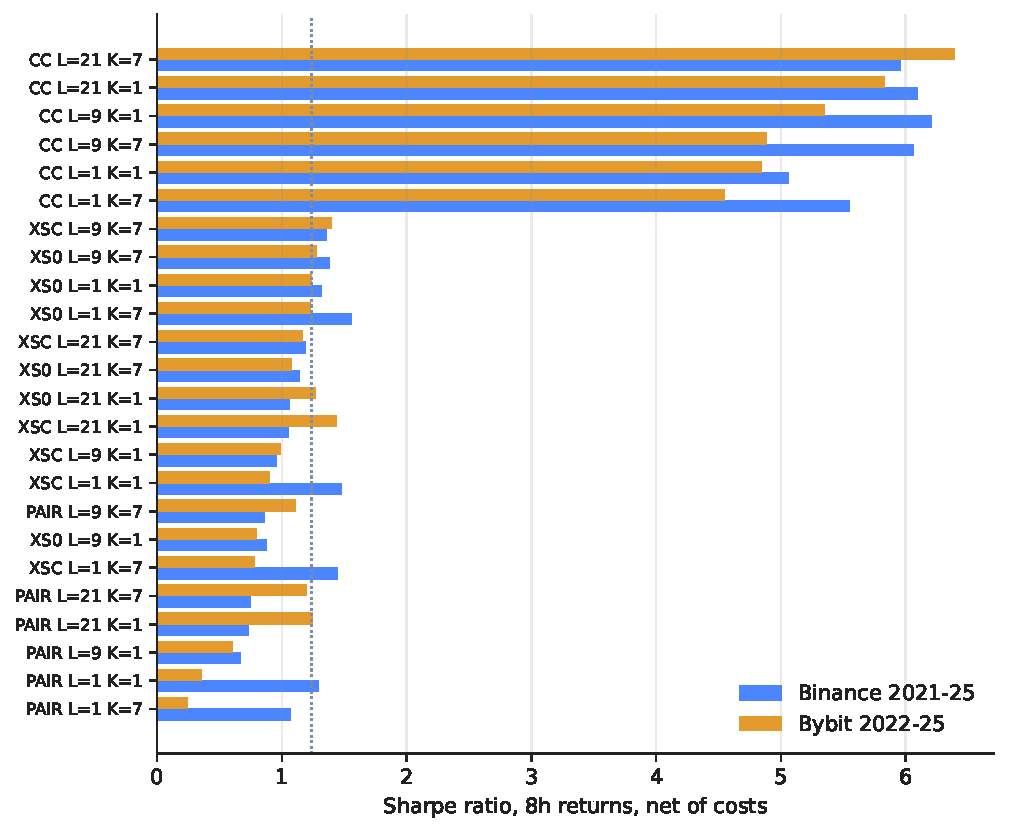
\includegraphics[width=0.82\linewidth]{sharpe_grid.pdf}
  \caption{All 24 configurations, sorted by the weaker venue. The dotted line is the
  baseline on Bybit. The four cash-and-carry configurations with smoothed signals sit
  far to the right; the other twenty cluster around the baseline.}
  \label{fig:grid}
\end{figure}

Figure~\ref{fig:grid} shows the full grid. Table~\ref{tab:r1} isolates each change
against the baseline. Only cash-and-carry improves on both venues; every other change
helps on one venue and hurts on the other, or hurts on both.

\begin{table}[h]
\centering\small
\caption{Each change on its own: difference in Sharpe ratio against the baseline
(XS0, $L=1$, $K=1$; \BnBaseSharpe{} on Binance, \ByBaseSharpe{} on Bybit).}
\label{tab:r1}
\begin{tabular}{lrr}
\toprule
Change & Binance & Bybit \\
\midrule
Signal: 3-day mean ($L=9$) & \ROneLNineBn & \ROneLNineBy \\
Signal: 7-day mean ($L=21$) & \ROneLTwentyOneBn & \ROneLTwentyOneBy \\
Seven tranches ($K=7$) & \ROneKSevenBn & \ROneKSevenBy \\
Inverse vol + BTC/ETH hedge (XSC) & \ROneXscBn & \ROneXscBy \\
Correlation pairs (PAIR) & \ROnePairBn & \ROnePairBy \\
\textbf{Cash-and-carry (CC)} & \textbf{\ROneCcBn} & \textbf{\ROneCcBy} \\
\bottomrule
\end{tabular}
\end{table}

The best combination inside the cross-sectional family, XSC with $L=9$ and $K=7$,
beats the baseline in-sample by a hair (\BnBestXsSharpe{} and \ByBestXsSharpe{}
against \BnBaseSharpe{} and \ByBaseSharpe). On the holdout it returned
\HoldBestXscTotal\%, against \HoldBaseTotal\% for the baseline. The best XS0 and PAIR
configurations returned \HoldBestXsZeroTotal\% and \HoldBestPairTotal\%. Smoothing and
tranching do reduce the dependence on the rebalance day: the standard deviation of the
final return across seven start days falls from \BnSchedBase{} to \BnSchedXsTwentyOne{}
percentage points on Binance. But they do not raise the Sharpe ratio reliably, because
they do not touch the dispersion bet.

\begin{figure}[h]
  \centering
  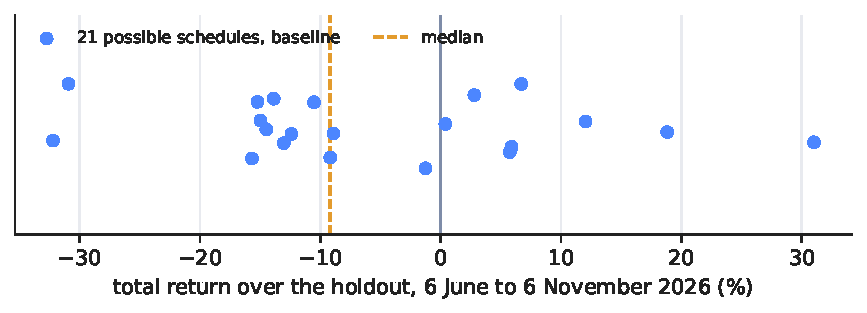
\includegraphics[width=0.82\linewidth]{holdout_schedules.pdf}
  \caption{The baseline on the five-month holdout, under each of its 21 possible
  schedules (7 start days times 3 funding times). Same rules, same coins available,
  outcomes from \HoldSchedLo\% to \HoldSchedHi\%.}
  \label{fig:sched}
\end{figure}

Figure~\ref{fig:sched} makes the point about evidence. Over the holdout, the baseline
ends anywhere from \HoldSchedLo\% to \HoldSchedHi\% depending only on which day and
funding time it rebalances on (median \HoldSchedMed\%; \HoldSchedNeg{} of 21 negative).
A single five-month result of the cross-sectional book carries very little
information. Cash-and-carry, by contrast, has a schedule spread of \BnSchedCc{} and
\BySchedCc{} points.

\subsection{Cash-and-carry: the right construction, in the wrong regime}

\begin{table}[h]
\centering\small
\caption{Baseline, best cross-sectional configuration and the selected candidate,
cash-and-carry with a 7-day signal and seven tranches. Sharpe on 8-hour returns, net
of costs.}
\label{tab:cand}
\begin{tabular}{lrrrrrr}
\toprule
 & \multicolumn{2}{c}{Sharpe} & \multicolumn{2}{c}{Return /yr} & \multicolumn{2}{c}{Max drawdown} \\
\cmidrule(lr){2-3}\cmidrule(lr){4-5}\cmidrule(lr){6-7}
 & Binance & Bybit & Binance & Bybit & Binance & Bybit \\
\midrule
Baseline XS0 $L{=}1$ $K{=}1$ & \BnBaseSharpe & \ByBaseSharpe & \BnBaseRet\% & \ByBaseRet\% & \BnBaseDD\% & \ByBaseDD\% \\
Best cross-sectional, XSC $L{=}9$ $K{=}7$ & \BnBestXsSharpe & \ByBestXsSharpe & \BnBestXsRet\% & \ByBestXsRet\% & \BnBestXsDD\% & \ByBestXsDD\% \\
\textbf{Cash-and-carry $L{=}21$ $K{=}7$} & \textbf{\BnCandSharpe} & \textbf{\ByCandSharpe} & \BnCandRet\% & \ByCandRet\% & \BnCandDD\% & \ByCandDD\% \\
\bottomrule
\end{tabular}
\end{table}

Cash-and-carry with a 7-day signal and seven tranches is selected without a tie and
passes the robustness rule (Table~\ref{tab:cand}). Its deflated Sharpe ratio over 48
trials is \Dsr{}. Holding the same coin long on spot and short on the perpetual removes
the dispersion bet by construction: what remains of the price leg is the basis between
spot and perpetual, and volatility falls from about 25\% to \ByCandVol\% a year on
Bybit.

The 8-hour Sharpe ratios overstate, because funding is persistent and the usual
$\sqrt{1095}$ annualisation assumes independent periods \cite{lo2002statistics}. On
monthly returns the Sharpe ratio is \BnCcMonthly{} (Binance) and \ByCcMonthly{}
(Bybit). That is still excellent. The problem is elsewhere.

\begin{figure}[h]
  \centering
  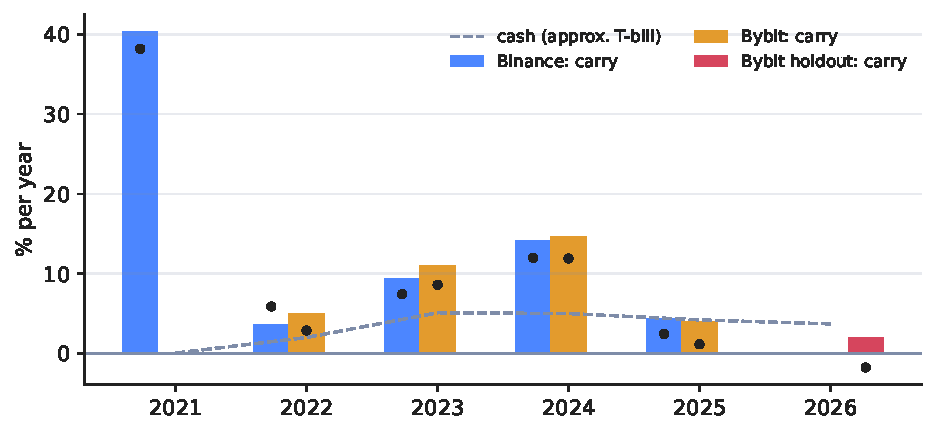
\includegraphics[width=0.82\linewidth]{cc_by_year.pdf}
  \caption{Cash-and-carry by calendar year: carry (bars) and net return after costs
  (dots), against an approximate cash yield (dashed). The return is the funding regime.}
  \label{fig:years}
\end{figure}

Figure~\ref{fig:years} shows it. The carry was \BnCcCarryTwentyOne\% in 2021, the leveraged
bull market, \BnCcCarryTwentyTwo\% in 2022, \BnCcCarryTwentyThree\% and \BnCcCarryTwentyFour\% in 2023
and 2024 (Binance), and then \BnCcCarryTwentyFive\% in 2025, below the cash yield of about
4\%. In the 2026 holdout it earned \HoCcCarryTwentySix\% a year in carry against
\HoldCandCost\% in costs, and returned \HoldCandTotal\% over five months. On Bybit the
return above cash over the whole sample is \ByCcExcess\% a year, and if spot cannot
serve as collateral for the short, capital roughly doubles and the return halves to
\ByCcSep\%, below cash. Funding is a price that leveraged longs pay for leverage. When
they stop demanding it, there is nothing to harvest.

Under the protocol cash-and-carry became a third live shadow ledger on 7 November,
next to the unchanged baseline and variant C. The honest expectation in the current
regime was roughly flat after costs.

\section{The live verdict}\label{sec:live}

\begin{figure}[t]
  \centering
  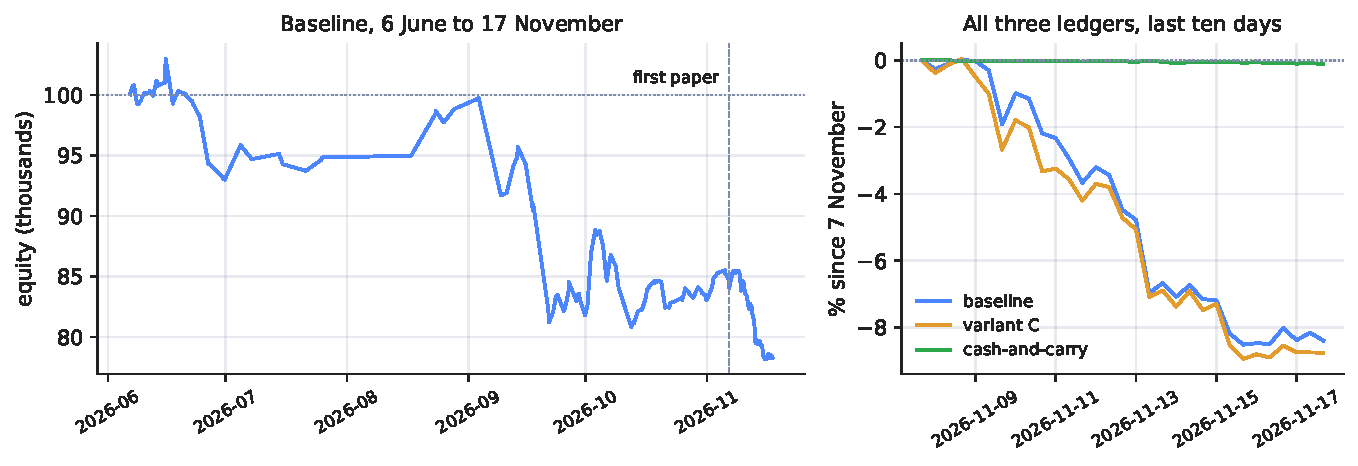
\includegraphics[width=\linewidth]{live_ledgers.pdf}
  \caption{Left: the baseline shadow ledger since 6 June. The dashed line marks the
  end of the first paper's window. Right: the three ledgers over the last ten days,
  rebased to 7 November. Baseline and variant C move together; cash-and-carry is flat.}
  \label{fig:live}
\end{figure}

\begin{table}[h]
\centering\small
\caption{The three live shadow ledgers on Bybit, up to \LiveEnd{}. The cross-sectional
ledgers charge no trading costs; the cash-and-carry ledger does.}
\label{tab:live}
\begin{tabular}{lrrr}
\toprule
 & Baseline & Variant C & Cash-and-carry \\
\midrule
Days live & \LiveDays & \CDays & \CcDays \\
Total return & \LiveTotal\% & \CTotal\% & \CcLiveTotal\% \\
Carry, cumulative & \LiveCarry\% & & \CcLiveCarry\% \\
Price, cumulative & \LivePrice\% & & \\
Carry, annualised & \LiveCarryAnn\% & & \CcLiveCarryAnn\% \\
\bottomrule
\end{tabular}
\end{table}

Table~\ref{tab:live} and Figure~\ref{fig:live} show the three ledgers. Since the first
paper the baseline lost a further \LiveSinceFirst\% in \LiveSinceFirstDays{} days, now
on the clean seven-day schedule and with price moves of only \LiveStepVol\% per
eight-hour step, a steady slide rather than a shock. It stands at \LiveTotal\% after
\LiveDays{} days, with carry of \LiveCarry\% and a price leg of \LivePrice\%.

\paragraph{Is the loss significant?} Using the standard error of the first paper,
$\sqrt{(1+\mathrm{SR}^2/2)/T}$, which allows for non-normal returns, the live Sharpe
ratio of \LiveSharpe{} against the Bybit backtest's \ByBaseSharpe{} gives
$z=\LiveZ$. The simpler standard error $1/\sqrt{T}$ gives $z=\LiveZNaive$. Of all
\LiveDays-day windows in the backtests, \BnWinNeg\% (Binance) and \ByWinNeg\% (Bybit)
lost money, but only \BnWinWorse\% and \ByWinWorse\% lost as much as the live ledger.
Against that, Figure~\ref{fig:sched} shows that the schedule alone spans more than 60
points over five months. The loss is unusual for the backtest, but it does not prove
on its own that the backtest was wrong.

\paragraph{Why the ledgers were frozen anyway.} The decision rests on economics, not on
the $z$-score:
\begin{enumerate}
  \item \textbf{Net of costs, the carry is about zero.} The live ledger charges no
  costs. Its carry of \LiveCarryAnn\% a year is the same as the \HoldBaseCost\% a year
  that the same book paid in trading costs over the holdout in the study engine, which
  leaves \LiveNetCarry{} points a year. What is left is the price leg.
  \item \textbf{The price leg is a bet without a demonstrated premium.} The first paper
  showed that its historical profit came from one or two 90-day windows; the first
  study showed that no construction makes it robust.
  \item \textbf{Variant C did not do its job.} Its eight-hour returns correlate
  \CCorr{} with the baseline, its price moves are no smaller (\CVol\% against
  \CBaseVol\% per step over the same window), and it returned \CTotal\% against
  \BaseSameWindow\% for the baseline. Lower risk was its only reason to exist.
  \item \textbf{More live data cannot change the decision.} With a schedule spread
  of this size, years of live data would be needed to separate a modest premium from
  noise, while the economics above are already known.
\end{enumerate}
The cross-sectional ledgers stopped advancing at 16:00 UTC on 17 November. Their files
are kept unchanged. The decision and its reasons were committed to the repository
before the second study was run, so that its outcome could not influence them.

\begin{quote}\small
\textbf{A correction.} The freeze note in the pre-registration of the second study
says the live loss is ``about two standard errors'' below the backtest. That figure
used the simple standard error. With the non-normality-adjusted standard error used
throughout this series it is \LiveZ. The note is left unchanged, as the protocol
requires; this paragraph is the correction.
\end{quote}

\section{The second study: a regime filter}\label{sec:study2}

\subsection{Protocol}

Cash-and-carry already leaves a slot empty when the smoothed funding is not positive.
But a coin earning 2\% a year still costs turnover and ties up capital that could earn
the cash yield. The second study, committed on 17 November before any test, adds one
parameter: a slot is filled only if the coin's 7-day mean funding, annualised, exceeds a
hurdle $\tau$. Four values are tested:

\begin{itemize}
  \item $\tau=0\%$: the live configuration, as control;
  \item $\tau=5\%$: roughly the cost of trading plus a margin;
  \item $\tau=10\%$: roughly costs plus the cash yield, just below the Bybit default
  rate of 10.95\%;
  \item $\tau=15\%$: only coins clearly above the default rate.
\end{itemize}

Capital not used for a spot leg earns the cash yield $c_t$ (approximate annual
averages of the 3-month US T-bill, 3.7\% assumed for 2026). With $g_t$ the share of
capital in use, the excess return over cash is
\begin{equation}
  x_t = \pi_t - g_t\,c_t ,
\end{equation}
the return the strategy adds over simply holding cash. The primary metric is the Sharpe
ratio of $x_t$. The candidate maximises the minimum of that Sharpe ratio across the two
venues, must beat $\tau=0$ on both, and is then evaluated once on the holdout. With
$\tau=0$ the modified engine reproduces the first study exactly, and a replay of the
live period reproduces the live cash-and-carry ledger to the cent.

\subsection{Results}

\begin{table}[h]
\centering\small
\caption{Cash-and-carry with an entry hurdle $\tau$. Excess is the return over cash.
Sharpe ratios of excess returns; ``in use'' is the average share of capital in a
position.}
\label{tab:tau}
\begin{tabular}{llrrrrr}
\toprule
$\tau$ & Venue & Sharpe (8h) & Sharpe (monthly) & Excess /yr & Cost /yr & In use \\
\midrule
0\%  & Binance & \TauZeroBnSharpe & \TauZeroBnMonthly & \TauZeroBnExcess\% & \TauZeroBnCost\% & \TauZeroBnGross\% \\
5\%  & Binance & \TauFiveBnSharpe & \TauFiveBnMonthly & \TauFiveBnExcess\% & \TauFiveBnCost\% & \TauFiveBnGross\% \\
10\% & Binance & \TauTenBnSharpe & \TauTenBnMonthly & \TauTenBnExcess\% & \TauTenBnCost\% & \TauTenBnGross\% \\
15\% & Binance & \textbf{\TauFifteenBnSharpe} & \TauFifteenBnMonthly & \TauFifteenBnExcess\% & \TauFifteenBnCost\% & \TauFifteenBnGross\% \\
\midrule
0\%  & Bybit & \TauZeroBySharpe & \TauZeroByMonthly & \TauZeroByExcess\% & \TauZeroByCost\% & \TauZeroByGross\% \\
5\%  & Bybit & \TauFiveBySharpe & \TauFiveByMonthly & \TauFiveByExcess\% & \TauFiveByCost\% & \TauFiveByGross\% \\
10\% & Bybit & \TauTenBySharpe & \TauTenByMonthly & \TauTenByExcess\% & \TauTenByCost\% & \TauTenByGross\% \\
15\% & Bybit & \textbf{\TauFifteenBySharpe} & \TauFifteenByMonthly & \TauFifteenByExcess\% & \TauFifteenByCost\% & \TauFifteenByGross\% \\
\bottomrule
\end{tabular}
\end{table}

The rule selects $\tau=15\%$ (Table~\ref{tab:tau}), which beats the control on both
venues and so counts as an improvement. On the holdout, evaluated once, the result is
stark: no coin cleared a 15\% hurdle in five months, so the book sat in cash
throughout, with an excess return of \HoTauFifteenExcess\% a year. The control earned
\HoTauZeroExcess\% a year against cash, the 5\% hurdle \HoTauFiveExcess\%, and the 10\%
hurdle, in a position \HoTauTenGross\% of the time, \HoTauTenExcess\%.

\begin{figure}[h]
  \centering
  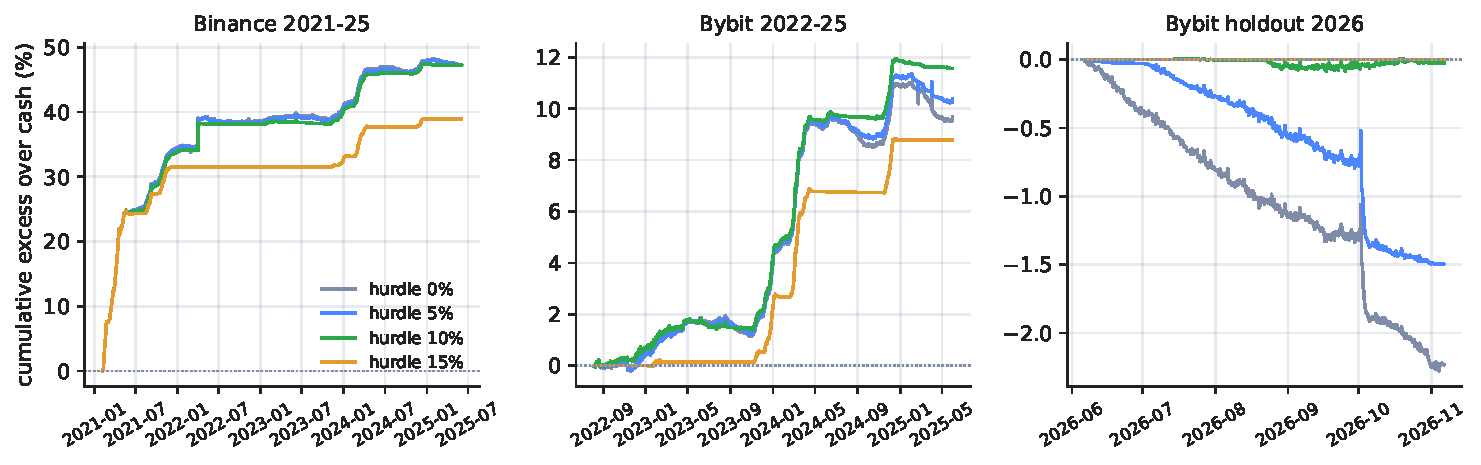
\includegraphics[width=\linewidth]{regime_excess.pdf}
  \caption{Cumulative excess return over cash for the four hurdles. In the good years
  all four earn about the same; the hurdles differ in the bad regimes, where the
  filtered books stand aside. Right: the holdout.}
  \label{fig:regime}
\end{figure}

\subsection{Reading the result honestly}

Three caveats keep this from being a stronger claim than it is.

\textbf{The primary metric flatters a book that is mostly in cash.} A period in cash
has an excess return of exactly zero, which lowers the volatility of 8-hour returns and
raises their Sharpe ratio. On monthly returns and on excess return per year, the 10\%
hurdle is slightly better than 15\% on both venues (monthly Sharpe \TauTenBnMonthly{}
and \TauTenByMonthly{} against \TauFifteenBnMonthly{} and \TauFifteenByMonthly).
The protocol chose 15\% and that choice stands; 10\% is reported as the more balanced
setting, not deployed.

\textbf{The filter avoids losses, it does not create returns.} Every hurdle earns
about the same in the good years (Figure~\ref{fig:regime}). On Bybit, the excess
return of the control by year was \YrZeroByB\%, \YrZeroByC\%, \YrZeroByD\% and
\YrZeroByE\% (2022 to 2025); with the 15\% hurdle it was \YrFifteenByB\%,
\YrFifteenByC\%, \YrFifteenByD\% and \YrFifteenByE\%. The gain is in 2025 and the
holdout, where the filter sits in cash instead of paying costs for carry below the cash
yield. It also gives up most of 2022.

\textbf{Small samples of bad regimes.} The hurdle is one parameter with a clear
economic meaning and four tested values, so the selection risk is small. But the
samples hold only one or two regimes in which carry fell below cash, which is exactly
the situation the filter is for.

Under rule R5 the 15\% hurdle runs as a fourth live shadow ledger from 18 November,
next to the unchanged cash-and-carry ledger. A replay of 7 to 17 November shows it would
have been in cash throughout. At the time of writing, funding was negative on most of
the 23 coins.

\section{Discussion}

\subsection{What the two studies support}

Three conclusions survive both pre-registered tests and the live evidence:

\begin{enumerate}
  \item \textbf{Cross-sectional funding books on a small universe are dispersion bets.}
  No construction tested here turns them into robust carry strategies, and their
  results depend on the rebalance schedule to a degree that makes months of live data
  nearly uninformative.
  \item \textbf{Cash-and-carry isolates the funding, and the funding is a regime.} It
  removes the dispersion almost completely, but what is left is the price leveraged
  longs pay. It was large in 2021 and 2024, and below cash in 2025 and 2026.
  \item \textbf{Cash is the right benchmark.} A book with 1 to 2\% volatility that earns
  4\% a year is not making money when cash pays 4\%. Measured against cash, standing
  aside in poor regimes is the main improvement available.
\end{enumerate}

\subsection{Lessons about method}

\textbf{Pre-registration changed the conclusions, not just the presentation.} The best
cross-sectional combination looked like a modest improvement in-sample and returned
\HoldBestXscTotal\%
on the holdout. Without a fixed rule for what counts as an improvement it would have
been easy to adopt it.

\textbf{Small implementation details move results.} Tie-breaking at the default
funding rate, and the rebalance day, each changed the cross-sectional book's results
by more than any of the intended design changes.

\textbf{Count costs in the live ledger.} The cross-sectional ledger reported carry
before costs, which made a book with zero net carry look like it was collecting
\LiveCarryAnn\% a year. The cash-and-carry ledgers charge costs from the start.

\subsection{Limitations}

\begin{itemize}
  \item \textbf{Short samples}: 4.3 and 2.8 years of backtest, holding few regimes of
  low funding.
  \item \textbf{Cash yields} are rounded annual averages, and 2026 is assumed.
  \item \textbf{Not modelled}: exchange and custody risk, auto-deleveraging,
  stablecoin risk, borrow limits, and intraperiod moves of the basis.
  \item \textbf{Fixed universe}: the 23 coins were chosen with hindsight from coins
  that are still liquid.
  \item \textbf{Shadow ledgers}: no orders were sent, so fills, slippage and funding
  accrual are modelled, not observed.
\end{itemize}

\section{Conclusion}

The funding on crypto perpetuals is a real cash flow, and the cleanest way to collect
it is cash-and-carry: short the perpetual, hold the coin. The cross-sectional book of
the first paper collected it too, but wrapped it in a dispersion bet that no hedge,
weighting or schedule could remove, and after \LiveDays{} days live its carry net of
costs was about zero. It has been frozen. Cash-and-carry earns what the market pays for
leverage, and in 2025 and 2026 the market paid less than cash. The one improvement
that survived pre-registration is not a better way to harvest funding but a rule for
when not to: hold a coin only while its funding clears a hurdle, and hold cash
otherwise. That is what now runs live.

\paragraph{Code and data.} Every number in this paper is generated by
\texttt{paper-regime/make\_assets.py} in the
\href{https://github.com/noaRoblesLevy/Quant-Research}{Quant-Research} repository
(project \texttt{funding-carry-harvest}). The pre-registrations are
\texttt{docs/preregistration\_2026-11-07.md} and
\texttt{docs/preregistration\_2026-11-17.md}; their commit times precede the results.

\paragraph{Disclaimer.} This is research, not investment advice. No real capital was
traded.

\begin{thebibliography}{9}
\setlength{\itemsep}{2pt}\small

\bibitem[Bailey and L\'opez de Prado(2014)]{bailey2014deflated}
D.~H. Bailey and M.~L\'opez de Prado.
\newblock The deflated Sharpe ratio: correcting for selection bias, backtest
  overfitting, and non-normality.
\newblock \emph{Journal of Portfolio Management}, 40(5):94--107, 2014.

\bibitem[Harvey et~al.(2016)]{harvey2016cross}
C.~R. Harvey, Y.~Liu, and H.~Zhu.
\newblock \ldots and the cross-section of expected returns.
\newblock \emph{Review of Financial Studies}, 29(1):5--68, 2016.

\bibitem[Koijen et~al.(2018)]{koijen2018carry}
R.~S.~J. Koijen, T.~J. Moskowitz, L.~H. Pedersen, and E.~B. Vrugt.
\newblock Carry.
\newblock \emph{Journal of Financial Economics}, 127(2):197--225, 2018.

\bibitem[Lo(2002)]{lo2002statistics}
A.~W. Lo.
\newblock The statistics of Sharpe ratios.
\newblock \emph{Financial Analysts Journal}, 58(4):36--52, 2002.

\end{thebibliography}

\end{document}
